\documentclass{tum_report}
% -----------------------------------------------------------------------
%  Extra packages that may not be in the template already
% -----------------------------------------------------------------------
\usepackage{amsmath}
\usepackage{amssymb}
\usepackage{float}
\usepackage{graphicx}
\usepackage{enumitem}
\usepackage{verbatim}
\usepackage{booktabs}
\usepackage{array}
\usepackage{xcolor}
\usepackage{hyperref}

\begin{document}

    \ministry{MINISTRY OF EDUCATION, CULTURE AND RESEARCH\\OF THE REPUBLIC OF MOLDOVA}


\university{\textbf{Technical University of Moldova}}
\faculty{\textbf{Faculty of Computers, Informatics and Microelectronics}}
\department{\textbf{Department of Software Engineering and Automatics}}

\title{Computer Graphics}

\year{2026}

\begin{titlepage}
    \centering

    % --- Logo ---
    
\includegraphics[width=0.25\textwidth]{./UTM_Logo.png}\par\vspace{1cm}

    % --- Ministry and University info ---
    {\bfseries
        \textsc{\ministryname} \\[0.15cm]
        \universityname\\[-0.01cm]
        \facultyname\\[-0.01cm]
        \departmentname
    }\par


    \vspace{2.5cm}

    % --- Student info ---
    \textbf{Mihail Pancenco} \textbf{FAF-243}\par

    \vspace{-0.5cm}

    % --- Title section ---
    {\Large \textbf{Report}\par} \normalsize	
    \vspace{0.5cm}
    {\normalfont\Large \textit{Laboratory work n. 1}\par}
    \vspace{-0.5cm}
    \Large \textit{of Operating Systems}\par \normalsize	

    \huge \textit{The OS as a Resource Manager}\par \normalsize	
    

    \vspace{3cm}

    % --- Checked by section ---
    \begin{flushright}
        {\normalfont
            Supervisers:\par
            \textbf{Dumitrașcu Marius}, \textit{University assistant}\par
            \textbf{Reițman Patricia}, \textit{University assistant}\par
            DISA, FCIM, UTM
        }
    \end{flushright}
    
    

    \vfill{}

    % --- Footer ---
    \textbf{Chișinău -- \degreeyear}\par

\end{titlepage}


    \clearpage

    \addtocontents{toc}{\protect \thispagestyle{empty}}
    \tableofcontents
    \thispagestyle{empty}
    \clearpage



% =======================================================================
\chapter{Introduction}
% =======================================================================

The goal of this laboratory work is to become familiar with xv6, a small
Unix-like teaching operating system. xv6 is a modern reimplementation of
Unix Version 6, containing the main components of a real operating system
while remaining small enough for its source code to be studied directly.

The operating system is built from source and executed on a RISC-V machine
provided by an emulator. This makes it possible to use xv6 as a small Unix
system, inspect both its user programs and kernel code, and run a program
written specifically for it.


\clearpage

% =======================================================================
\chapter{Before we start}
% =======================================================================

The work is performed in an Ubuntu virtual machine running in VirtualBox.
The Ubuntu system itself runs on the ARM64 architecture, while xv6 is built
for RISC-V.

RISC-V is an open instruction set architecture developed at the University
of California, Berkeley. Its development began in 2010 as a new architecture
for computer architecture research and processor design. The name refers to
the fifth generation of the Berkeley RISC architecture lineage.

An instruction set architecture defines the machine instructions understood
by a processor together with fundamental aspects of its programming model.
RISC-V can therefore be implemented by physical processors as well as by
software emulators. xv6 uses RISC-V as its target architecture, independently
of the architecture on which the development tools themselves are running.

Since Ubuntu is running on ARM64 while the generated xv6 code must contain
RISC-V instructions, a RISC-V cross-compilation toolchain is used. The
\texttt{riscv64-linux-gnu-gcc} compiler translates C source files into
object files containing 64-bit RISC-V machine code.

The separate object files are then combined by
\texttt{riscv64-linux-gnu-ld}. The linker resolves references between them
and produces the binaries that form the kernel and user programs. The linker,
assembler, \texttt{objdump}, \texttt{objcopy}, and several related tools are
provided by GNU Binutils for RISC-V.

The build sequence is controlled by GNU Make according to the rules stored
in the xv6 \texttt{Makefile}. It invokes the required compilation and linking
commands and provides targets for building and starting the system.

The resulting RISC-V machine code cannot be executed directly by the ARM64
processor used by Ubuntu. QEMU provides the required RISC-V system in
software. The \texttt{qemu-system-riscv64} emulator represents a complete
64-bit RISC-V computer on which xv6 can boot and execute.

The execution environment therefore consists of several layers:

\begin{center}
Physical computer
$\rightarrow$
VirtualBox
$\rightarrow$
Ubuntu ARM64
$\rightarrow$
QEMU RISC-V
$\rightarrow$
xv6.
\end{center}

GDB Multiarch is also part of the development toolchain. It can debug programs
for architectures other than that of the host machine and can be connected
to an emulated RISC-V system to inspect execution, memory, processor
registers, and kernel state.

The xv6 sources are expected to be stored in
\texttt{\textasciitilde/xv6-riscv}. To begin, we will look for this directory
in the home folder.


\begin{figure}[H]
    \centering
    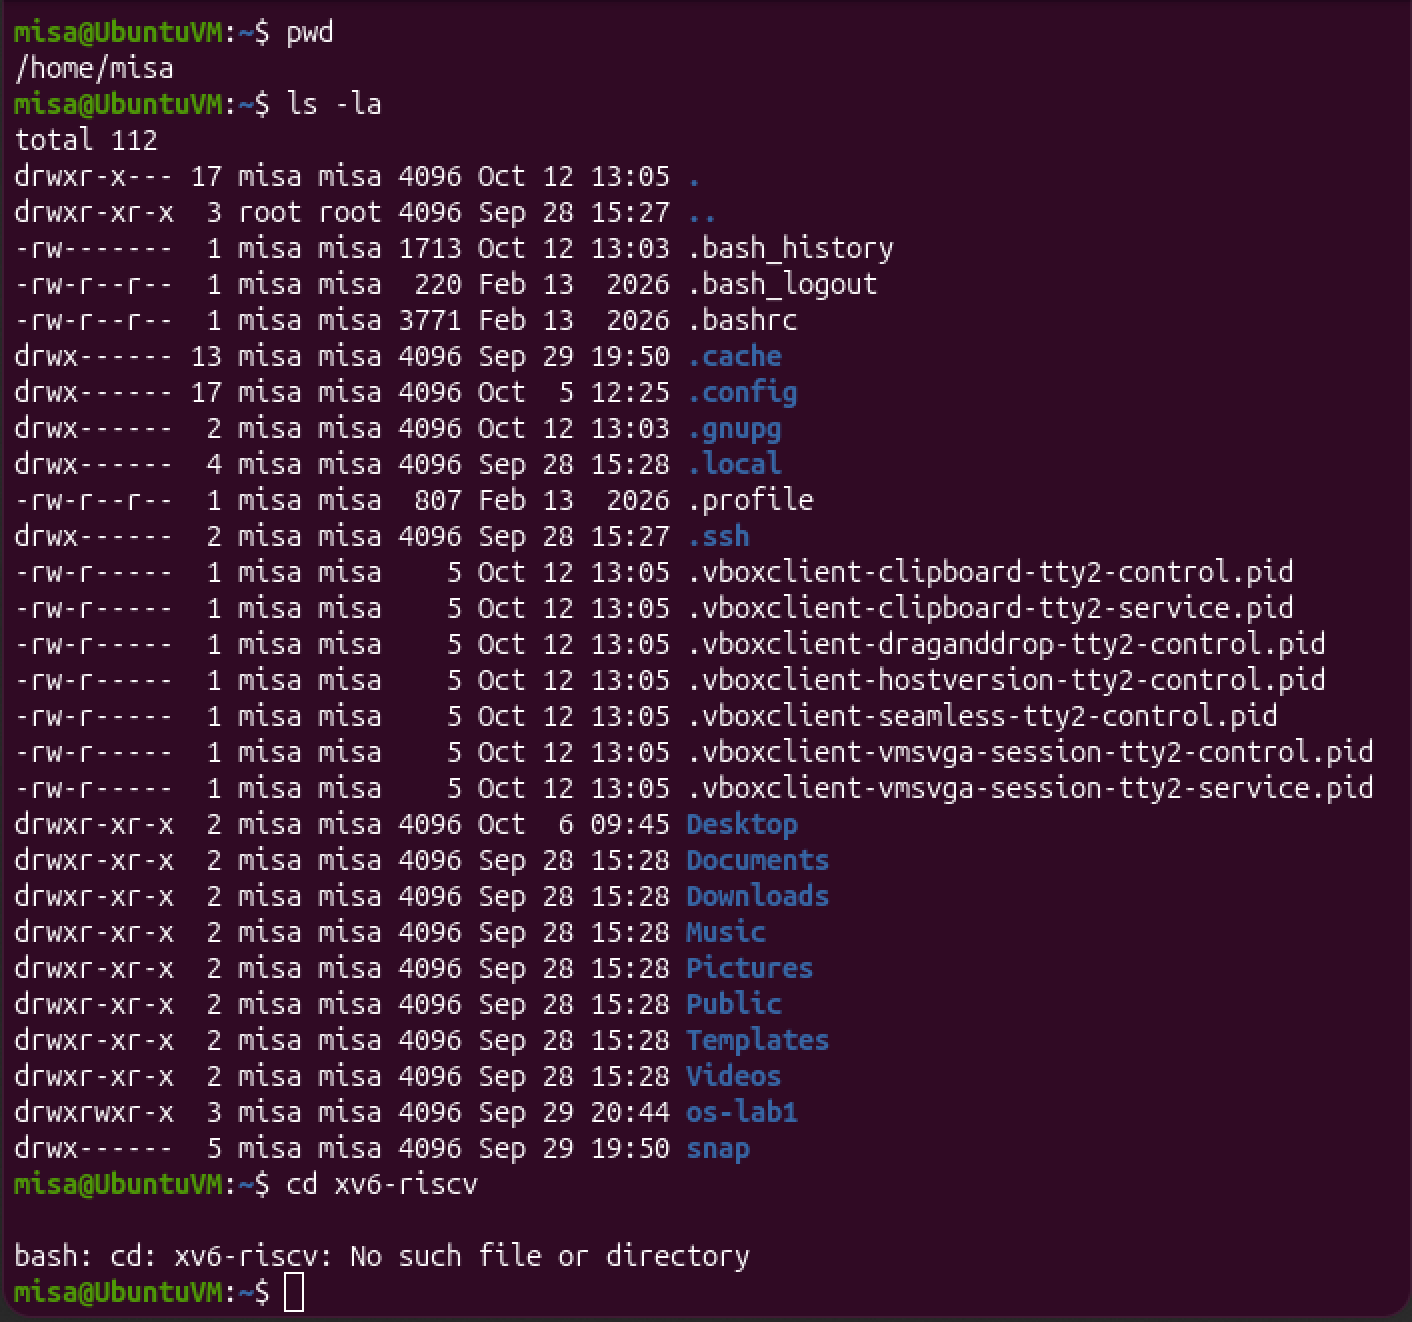
\includegraphics[width=0.82\textwidth]{./img/img_01.png}
    \caption{Checking the home directory for the xv6 source code}
    \label{fig:xv6_directory_check}
\end{figure}

The \texttt{xv6-riscv} directory is not present in the home folder, so the
xv6 source code still needs to be obtained.

Before obtaining the source code, we check whether the tools required to
build and run xv6 are available.

\begin{figure}[H]
    \centering
    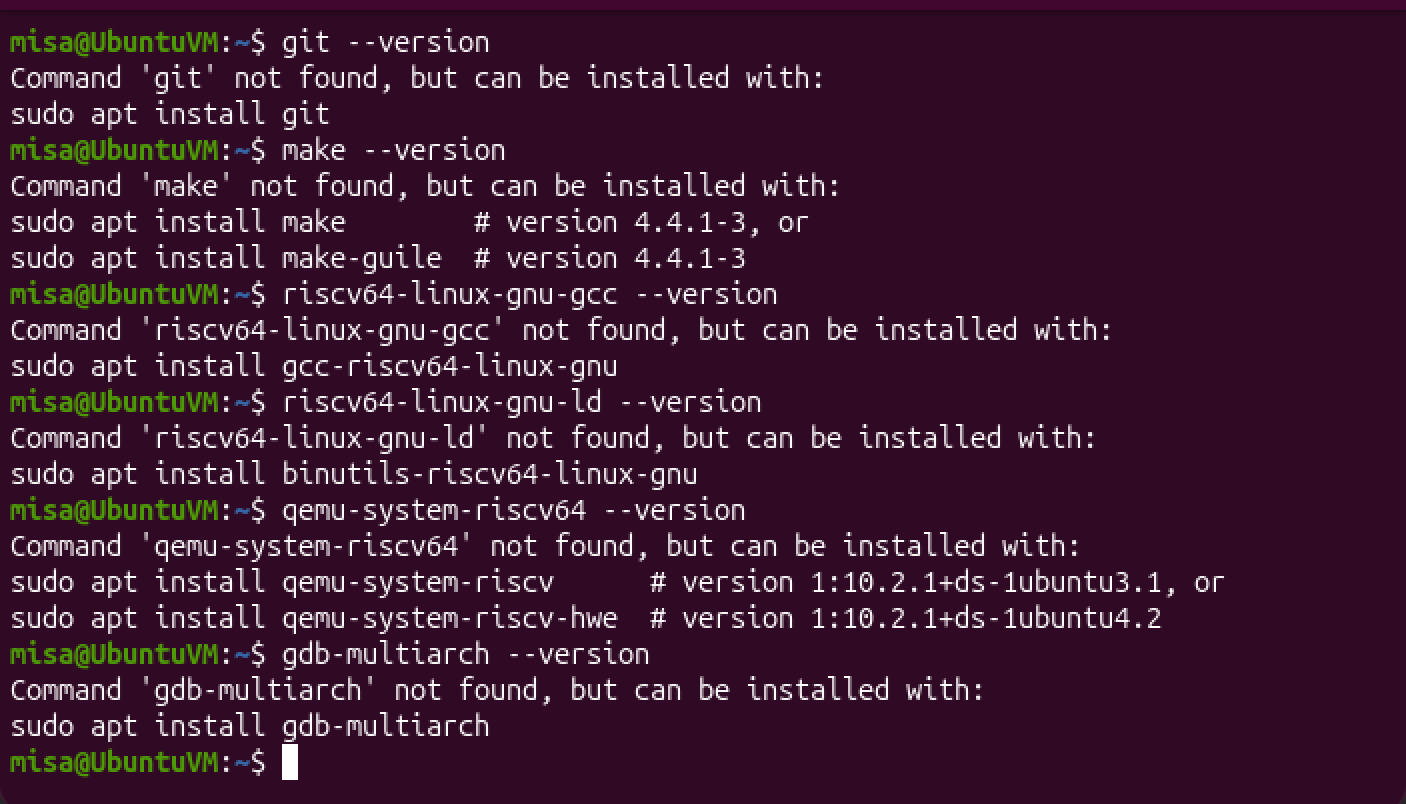
\includegraphics[width=0.82\textwidth]{./img/img_02.png}
    \caption{Checking the availability of the required development tools}
    \label{fig:toolchain_check}
\end{figure}

None of the required tools are currently available in the system. The
development environment therefore needs to be prepared before xv6 can be
built and executed.

The missing tools are installed through the Ubuntu package manager.

\begin{figure}[H]
    \centering
    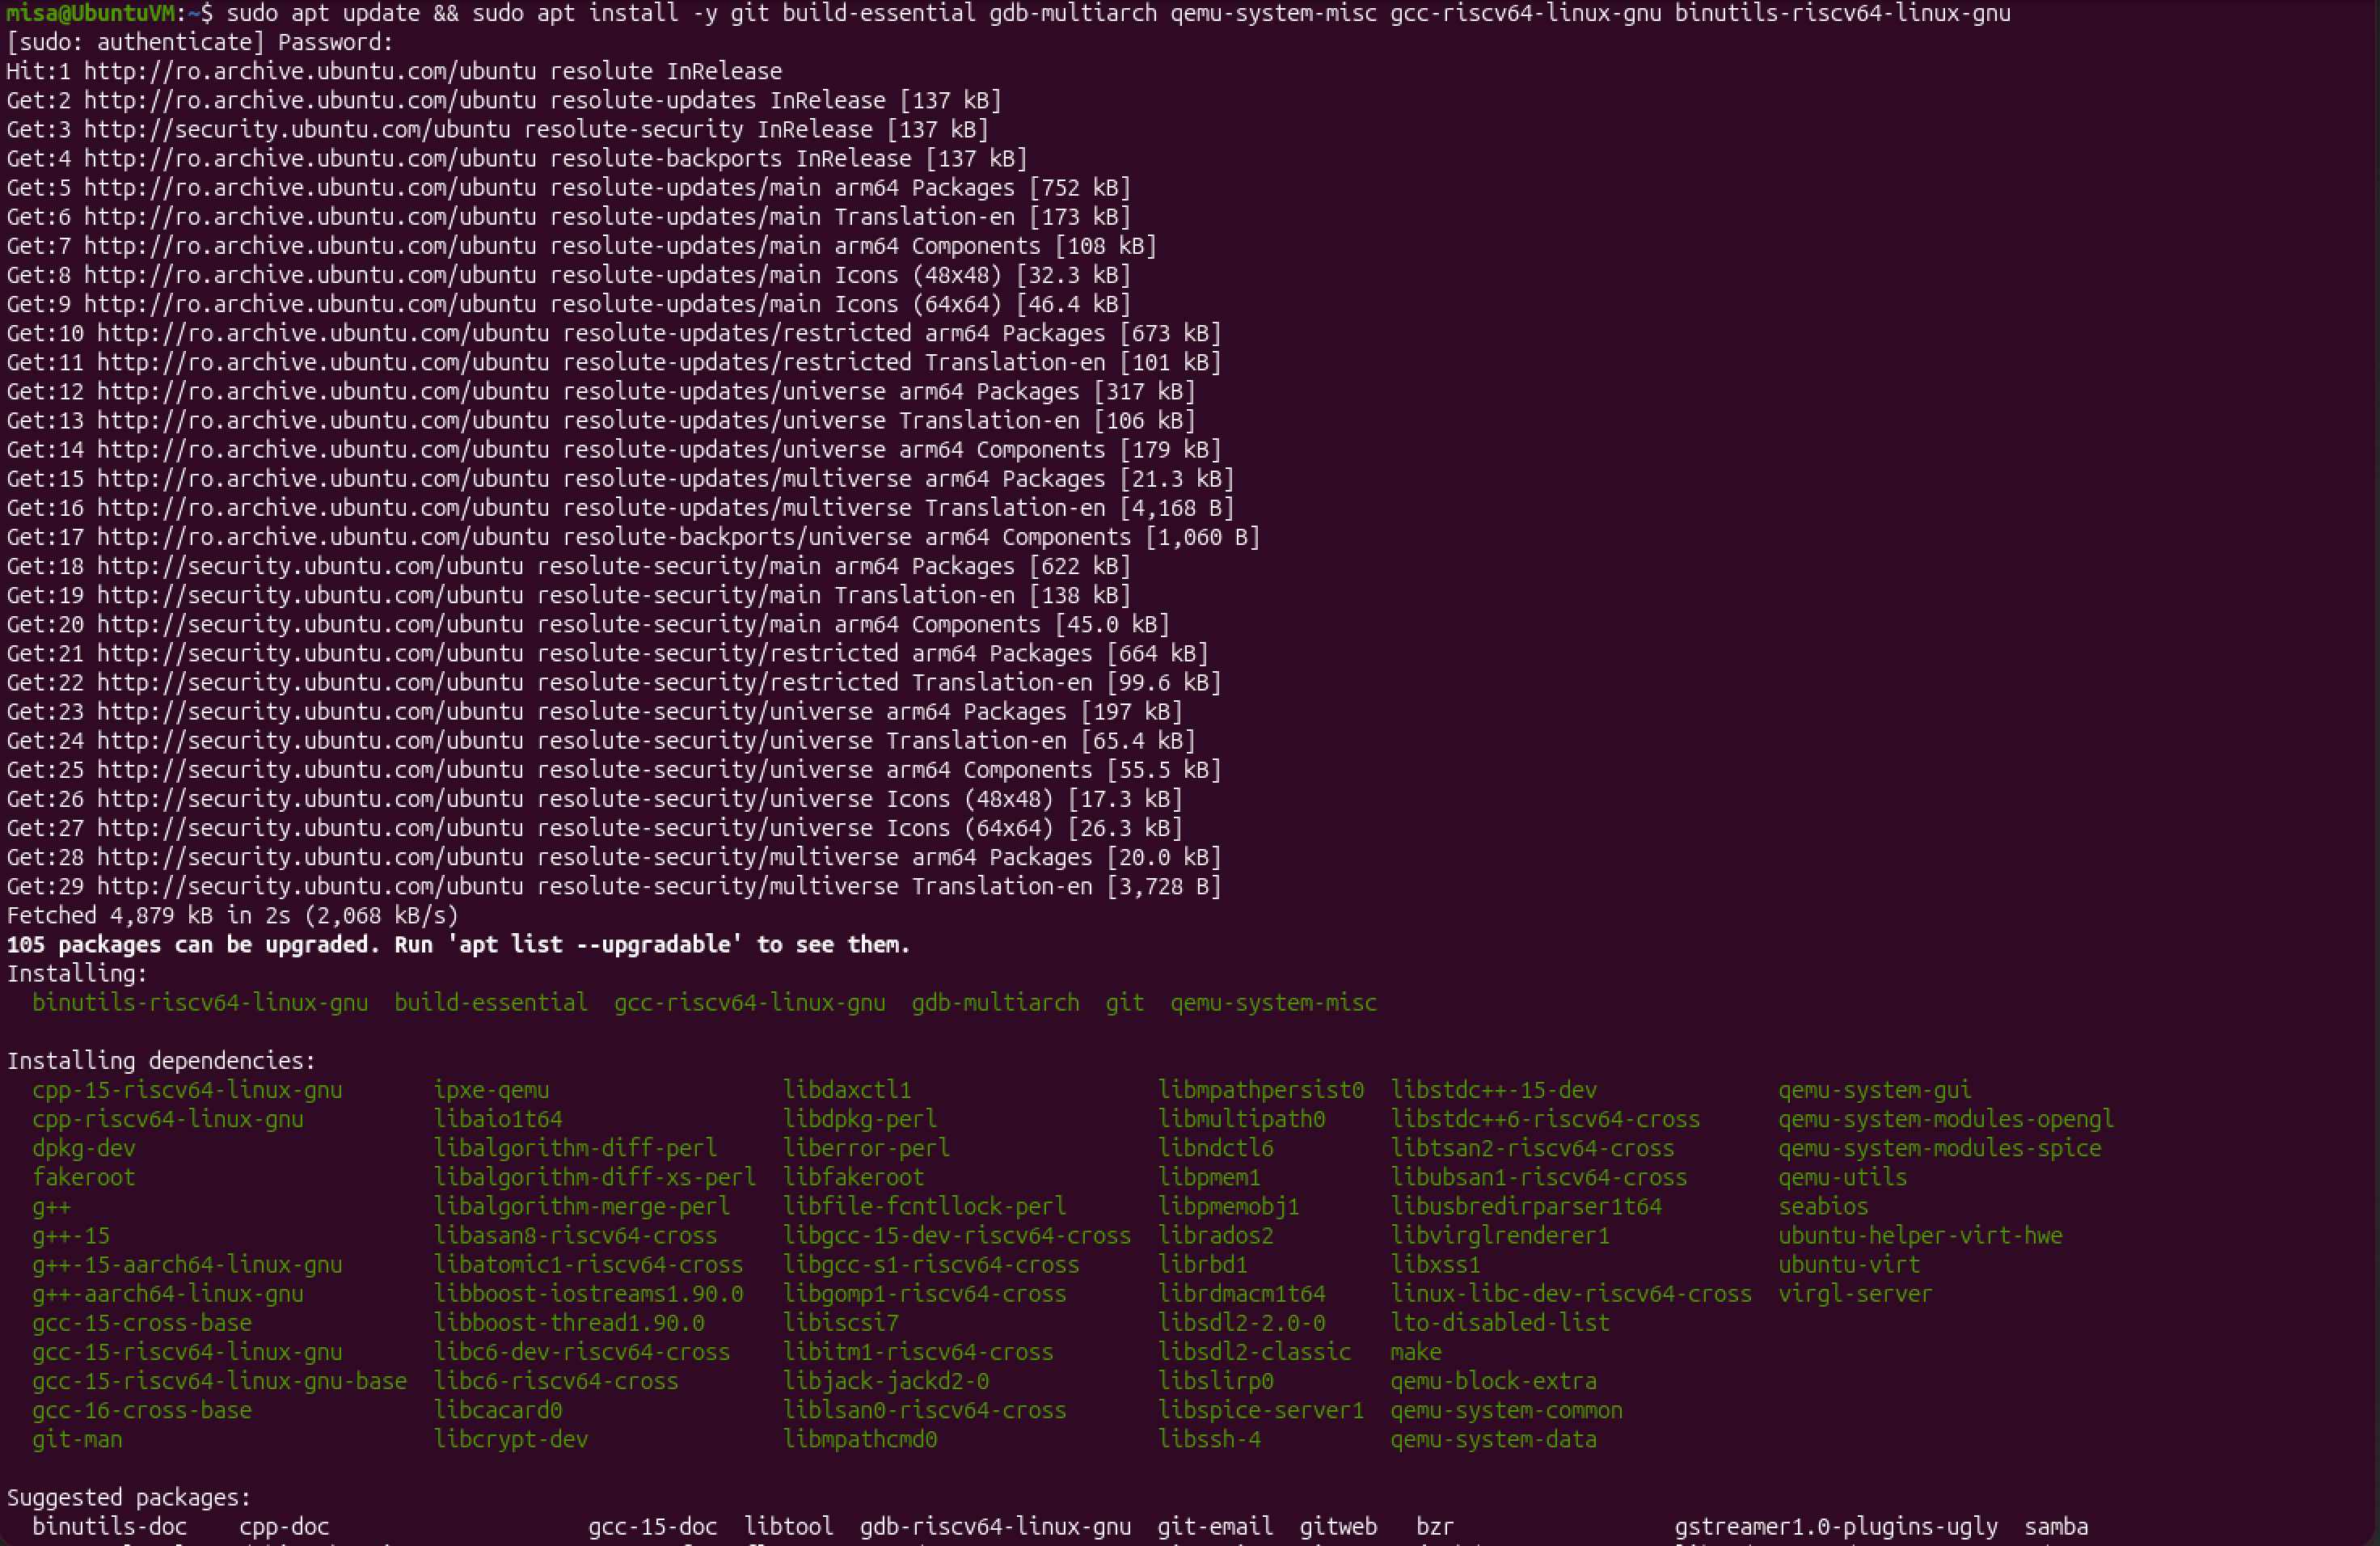
\includegraphics[width=0.82\textwidth]{./img/img_03.png}
    \caption{Installing the xv6 development toolchain}
    \label{fig:toolchain_installation}
\end{figure}

The installed tools were then checked again.

\begin{figure}[H]
    \centering
    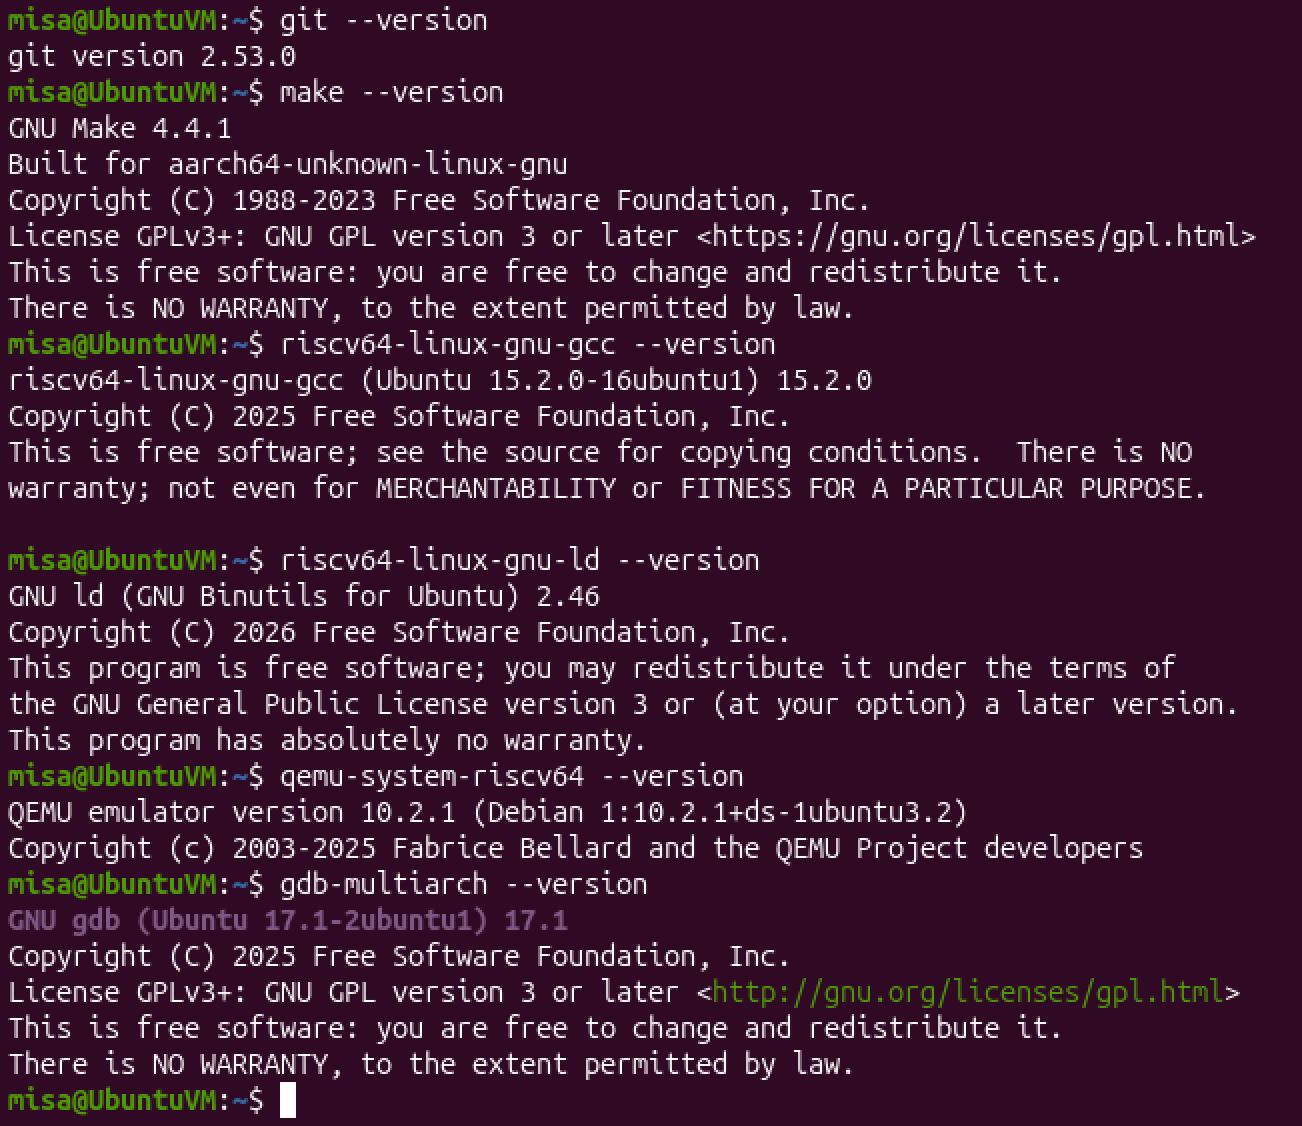
\includegraphics[width=0.82\textwidth]{./img/img_04.png}
    \caption{Verification of the installed development tools}
    \label{fig:toolchain_verification}
\end{figure}

All required development tools are now installed and available in the system.
The environment is ready for working with xv6.

With the development environment ready, the xv6 source code can now be
obtained from the official repository.

\begin{figure}[H]
    \centering
    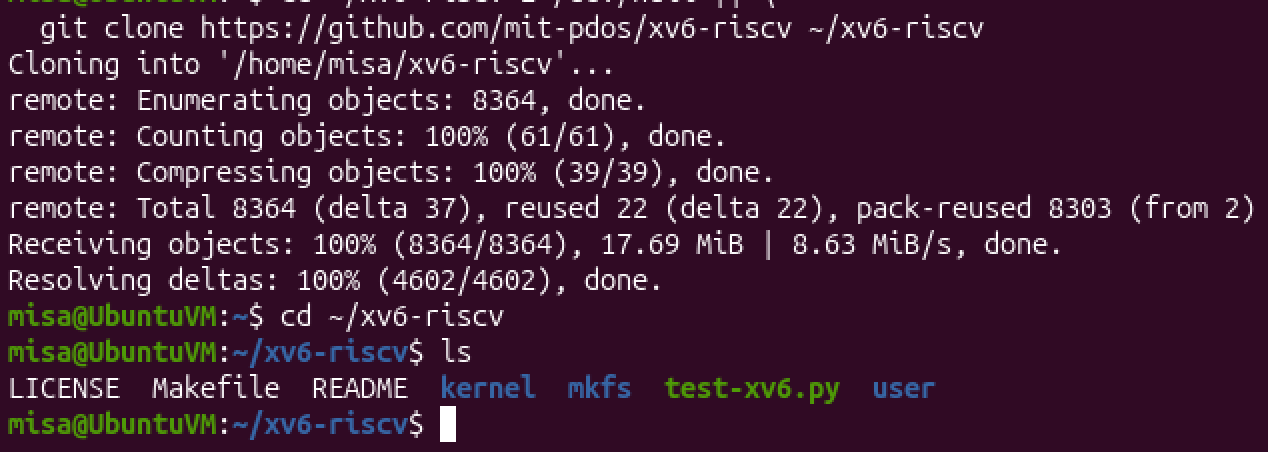
\includegraphics[width=0.82\textwidth]{./img/img_05.png}
    \caption{Cloning and inspecting the xv6 source repository}
    \label{fig:xv6_repository}
\end{figure}

The xv6 source tree is now available in
\texttt{\textasciitilde/xv6-riscv}. It contains the kernel sources, user
programs, the Makefile, and the other files required to build the system.


\chapter{Building the OS}
\section{Build it and boot it}

The xv6 kernel and user programs were built from source using the RISC-V
toolchain. Make compiled and linked the required components, created the
filesystem image, and launched the resulting system in QEMU.

\begin{figure}[H]
    \centering
    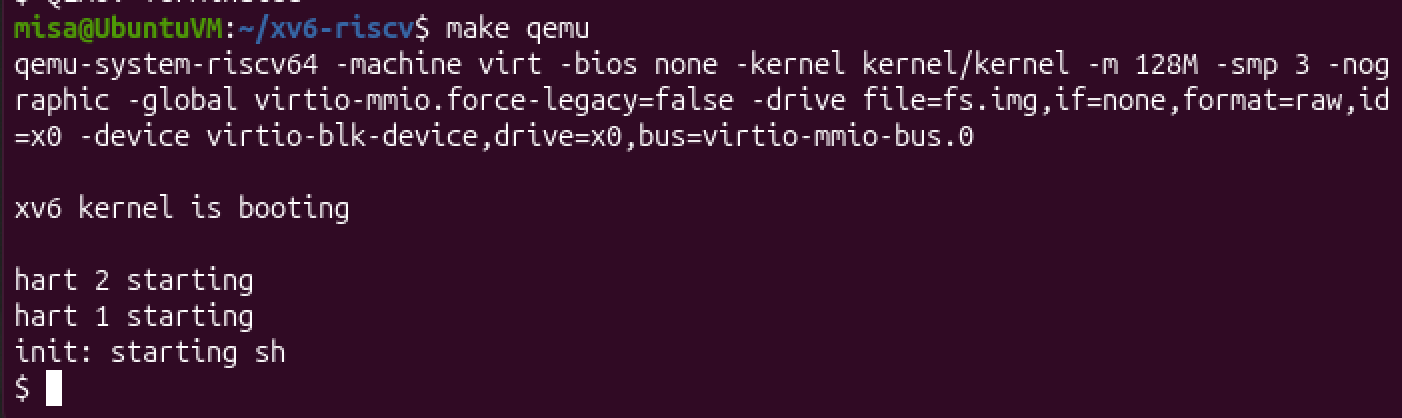
\includegraphics[width=0.82\textwidth]{./img/img_06.png}
    \caption{Booting xv6 in the QEMU RISC-V emulator}
    \label{fig:xv6_boot}
\end{figure}

The boot completed successfully. After initializing the system, xv6 started
its shell and presented the command prompt.



\section{Use xv6 as the Unix it is}
\section{Read the source}
\section{Write first xv6 program}





\clearpage

% =======================================================================
\chapter{CONCLUSIONS}
% =======================================================================


% =======================================================================
% =======================================================================


\clearpage

% =======================================================================
% Bibliography
% =======================================================================

%\begin{thebibliography}{99}
\singlespace \normalsize

% \bibitem{ref:Chicago}
%   The Chicago Manual of Style.
%   "Notes and Bibliography: Sample Citations".
%   Accessed October 14, 2022.
%   \url{https://www.chicagomanualofstyle.org/tools_citationguide/citation-guide-2.html}.

% \bibitem{ref:Cats}
%   Google.
%   "Search results for cats".
%   Accessed August 15, 2023.
%   \url{https://www.google.com/search?q=cats}.

\bibitem{ref:OS-GfG}
  GeeksforGeeks.
  "What is an Operating System?".
  Last Updated July 25, 2025.
  Accessed October 16, 2025.
  \url{https://www.geeksforgeeks.org/operating-systems/what-is-an-operating-system/}.

\bibitem{ref:OS-concept}
Silberschatz, A., Galvin, P. B., \& Gagne, G. (2018).
\textit{Operating System Concepts} (10th ed.).
Wiley.
ISBN 978-1-119-32091-3.

\end{thebibliography}



\clearpage
\end{document}
